\documentclass{standalone}
\usepackage{pgfplots}
\pgfplotsset{compat=1.16}

\begin{document}
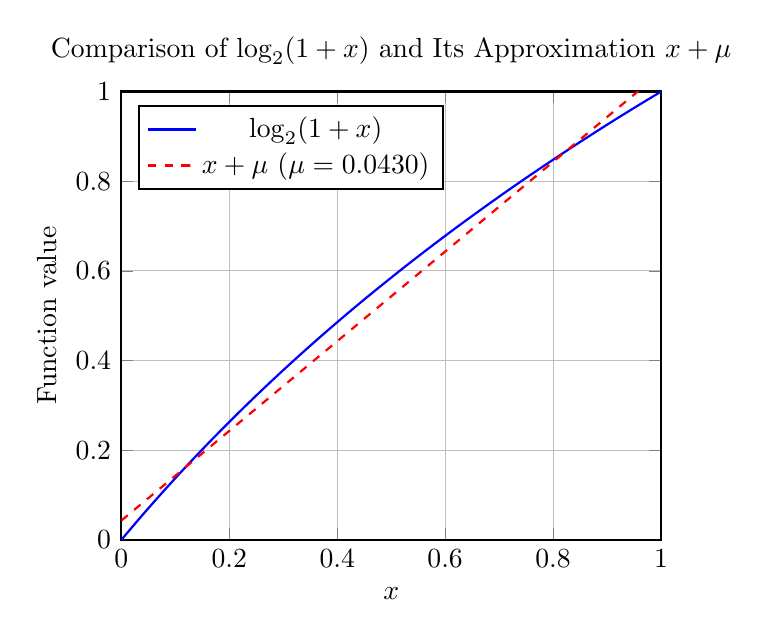
\begin{tikzpicture}
\begin{axis}[
    title={Comparison of $\log_2(1 + x)$ and Its Approximation $x + \mu$},
    xlabel={$x$},
    ylabel={Function value},
    legend pos=north west,
    grid=major,
    thick,
    xmin=0, xmax=1, % Ustawienie zakresu osi x od 0 do 1
    domain=0:1, % Zakres wartości x używanych dla funkcji
    ymin=0, ymax=1 % Opcjonalnie ogranicz zakres wartości y, jeśli potrzebny
]
% Add plots
\addplot[blue, smooth] {log2(1 + x)};
\addlegendentry{$\log_2(1 + x)$}

\addplot[red, smooth, dashed] {x + 0.0430};
\addlegendentry{$x + \mu$ ($\mu=0.0430$)}
\end{axis}
\end{tikzpicture}
\end{document}

